% ===========================================
% Project 3: 7-Segment Display Counter
% Written by: Braidan Duffy
%
% Date: 05/26/2022
% Last Revision: 08/25/2022
% ============================================

\chapter{Project 3: 7-Segment Display Counter}
\labch{p3_7seg_counter}

\section*{Overview}
This project will introduce you to the shift register, the seven segment display, and the active piezoelectric buzzer.
You will incorporate many of the lessons previously learned including digital inputs and filtering, interrupts, digital outputs, mode selection, and counting.

\section*{Undergraduate Students}
You will only be focussed on working with the four digit seven segment display counter.
You wire up the display with the 74HC595 shift register IC and increment the display based on the current millisecond reading of the Arduino since time on \emph{or} a count reset button press.
When the reset count button is pressed, the counter will reset back to 0 and a buzzer will sound for auditory feedback.

\marginnote{In decimal, the display can only display up to four non-negative digits meaning you can only display a maximum of 9999. 
Make sure your code is capable of resetting the counter when this value is reached. 
\emph{For extra credit:} figure out how to make it count higher than 9999.} 

For heaps of extra credit, you may elect to do the \hyperref[sec:p3_grad_students]{graduate student section} of this project.

Since this project is more complicated than previous ones, the schematic for the breadboard and the psuedocode are provided in this document. It is \emph{strongly} suggested you start this project early and do not wait to work on it.

    \subsection*{Requirements}
    For this project you will be required to have the following:
    \begin{enumerate}
        \item A button wired to an interrupt-capable input
            \begin{itemize}
                \item These buttons will be attached to digital interrupts to trigger the counter reset and sound a buzzer
                \marginnote{\emph{For extra credit:} Figure out how to change the buzzer's volume without changing the circuit every time}
            \end{itemize}
        \item The current counter value will be displayed on a 4-digit, 7-segment display
        \item A "neat" breadboard where wires are easy to track, components are visible, cross jumps are minimized, and wire colors are somewhat sensible (i.e. all orange for the shift register, white for digit selectors, etc.).
    \end{enumerate}

    \subsection*{Submission}
    You will be required to submit the following on Canvas:
    \begin{enumerate}
        \item the source code file
        \item a picture of your Arduino and breadboard set up.
    \end{enumerate}

    \subsection*{Grading}
    You will be graded along the following criteria:

    \begin{margintable}[-0.5in]
        \begin{tabular}{ l | c }
            \toprule
            Criterion & Points \\

            \midrule
            Efficacy & 70 \\
            Breadboard neatness & 10 \\
            Code neatness & 20 \\
            Extra credit & 10 \\

            \bottomrule
        \end{tabular}
    \end{margintable}

    If you are willing to dig in a little bit more, this project has a couple of opportunities to earn extra credit points!
    If you want to try and get the extra credit points, please let the instructor know in the submission and detail why you believe you earn the points.

    \subsection*{Miscellanea}
    Since working with bits and registers and 7-segment displays can be tricky for beginners, the binary sequences for various numbers and letters are provided in the table below. Note that these values will change depending on how the shift register is wired to the 7-segment display. The values provided are known and tested to have worked with the schematics shown above.

    \begin{margintable}[-1.5in]
        \begin{tabular}{c | c}
            \toprule
            Character & Hex Code \\

            \midrule
            0 & 0x3F \\
            1 & 0x06 \\
            2 & 0x5B \\
            3 & 0x4F \\
            4 & 0x66 \\
            5 & 0x6D \\
            6 & 0x7D \\
            7 & 0x07 \\
            8 & 0x7F \\
            9 & 0x6F \\
            A & 0x77 \\
            b & 0x7c \\
            C & 0x39 \\
            d & 0x5E \\
            E & 0x79 \\
            F & 0x71 \\
                & 0x00 \\

            \bottomrule
        \end{tabular}
    \end{margintable}

    \pagelayout{wide} % Remove margins

    \subsection*{Pseudocode}
    \begin{lstlisting}[linewidth=1.5\textwidth]
Program: 4-Digit 7-Segment Display Counter

Define the 74HC595 data pin as some Arduino pin
Define the 74HC595 latch pin as some Arduino pin
Define the 74HC595 clock pin as some Arduino pin
Define the digit control pins as an array of some Arduino pins
Initialize the display digital values as an array of values with Digit One being index 0 (MSB last)

Initialize an array of hex values corresponding to letters and numbers

Define the button reset pin on some interrupt-capable Arduino pin

Define the buzzer pin as some Arduino pin
Define the buzzer active time as some time in milliseconds
Initialize the buzzer active flag as false
Initialize the buzzer start time as 0

Initialize the start time as 0 or the current millisecond value

Function: Setup
    Set up 7-segment display pins as outputs
    Set up button input pin as an input pullup
    Attach the counter reset ISR function to the button input to trigger on the falling edge
    Set up the buzzer output pin
    Set the buzzer output pin to LOW to ensure buzzer is off

Function: Loop
    Update the display
    If one second has passed since the last execution then
        Reset execution timer
        update the counter
    
    If the buzzer active flag is true then
        If the buzzer active time has not elapsed then
            Turn the buzzer on
        Else
            Set the buzzer active flag to false
            Turn off the buzzer

Function: Turn off Display
    For every pin in the digit display pins array
        Set the pin to low to turn off the digit

Function: Display
    Arguments: Index of value to be displayed, found in the table of values
    Set the latch pin to low to enable shift register writing
    Shift out the value of table at the specified index to the shift register
    Set the latch pin to high to disable shift register writing

Function: Update Display
    For every digit in the display digits array
        Turn off the display
        Display the value of the current digit
        Turn on the specific digit in the display
        Delay a little bit to give everything time to process (~1 ms)
    Turn off the display to reduce power consumption

Function: Update Counter
    If every digit in the digit display array is equal to 9 then
        Reset every value in the digit display array to 0
        
    Initialize the an increment value flag as true
    For every digit in the digit display array
        Store the value of the specific digit in a temporary variable
        If the increment value flag is true then
            Increment the temporary variable by one
            Set the increment value flag to false
            If the temporary variable is greater than 9 then
                Reset the specific digit to 0
                Set the increment value flag to true
            Else
                Set the specific digit to the new value of the temporary variable

Function: Counter Reset ISR
    For every digit in the display digits array
        Set the specific digit value to 0
    Set the buzzer active flag to true
    Set the buzzer start time to the current millisecond value
    \end{lstlisting}

    \subsection*{Schematic}
    \begin{figure*}[ht!]
        \labfig{p3_7seg_counter_bb_ugrad}
        \caption{Breadboard schematic for Project 3}
        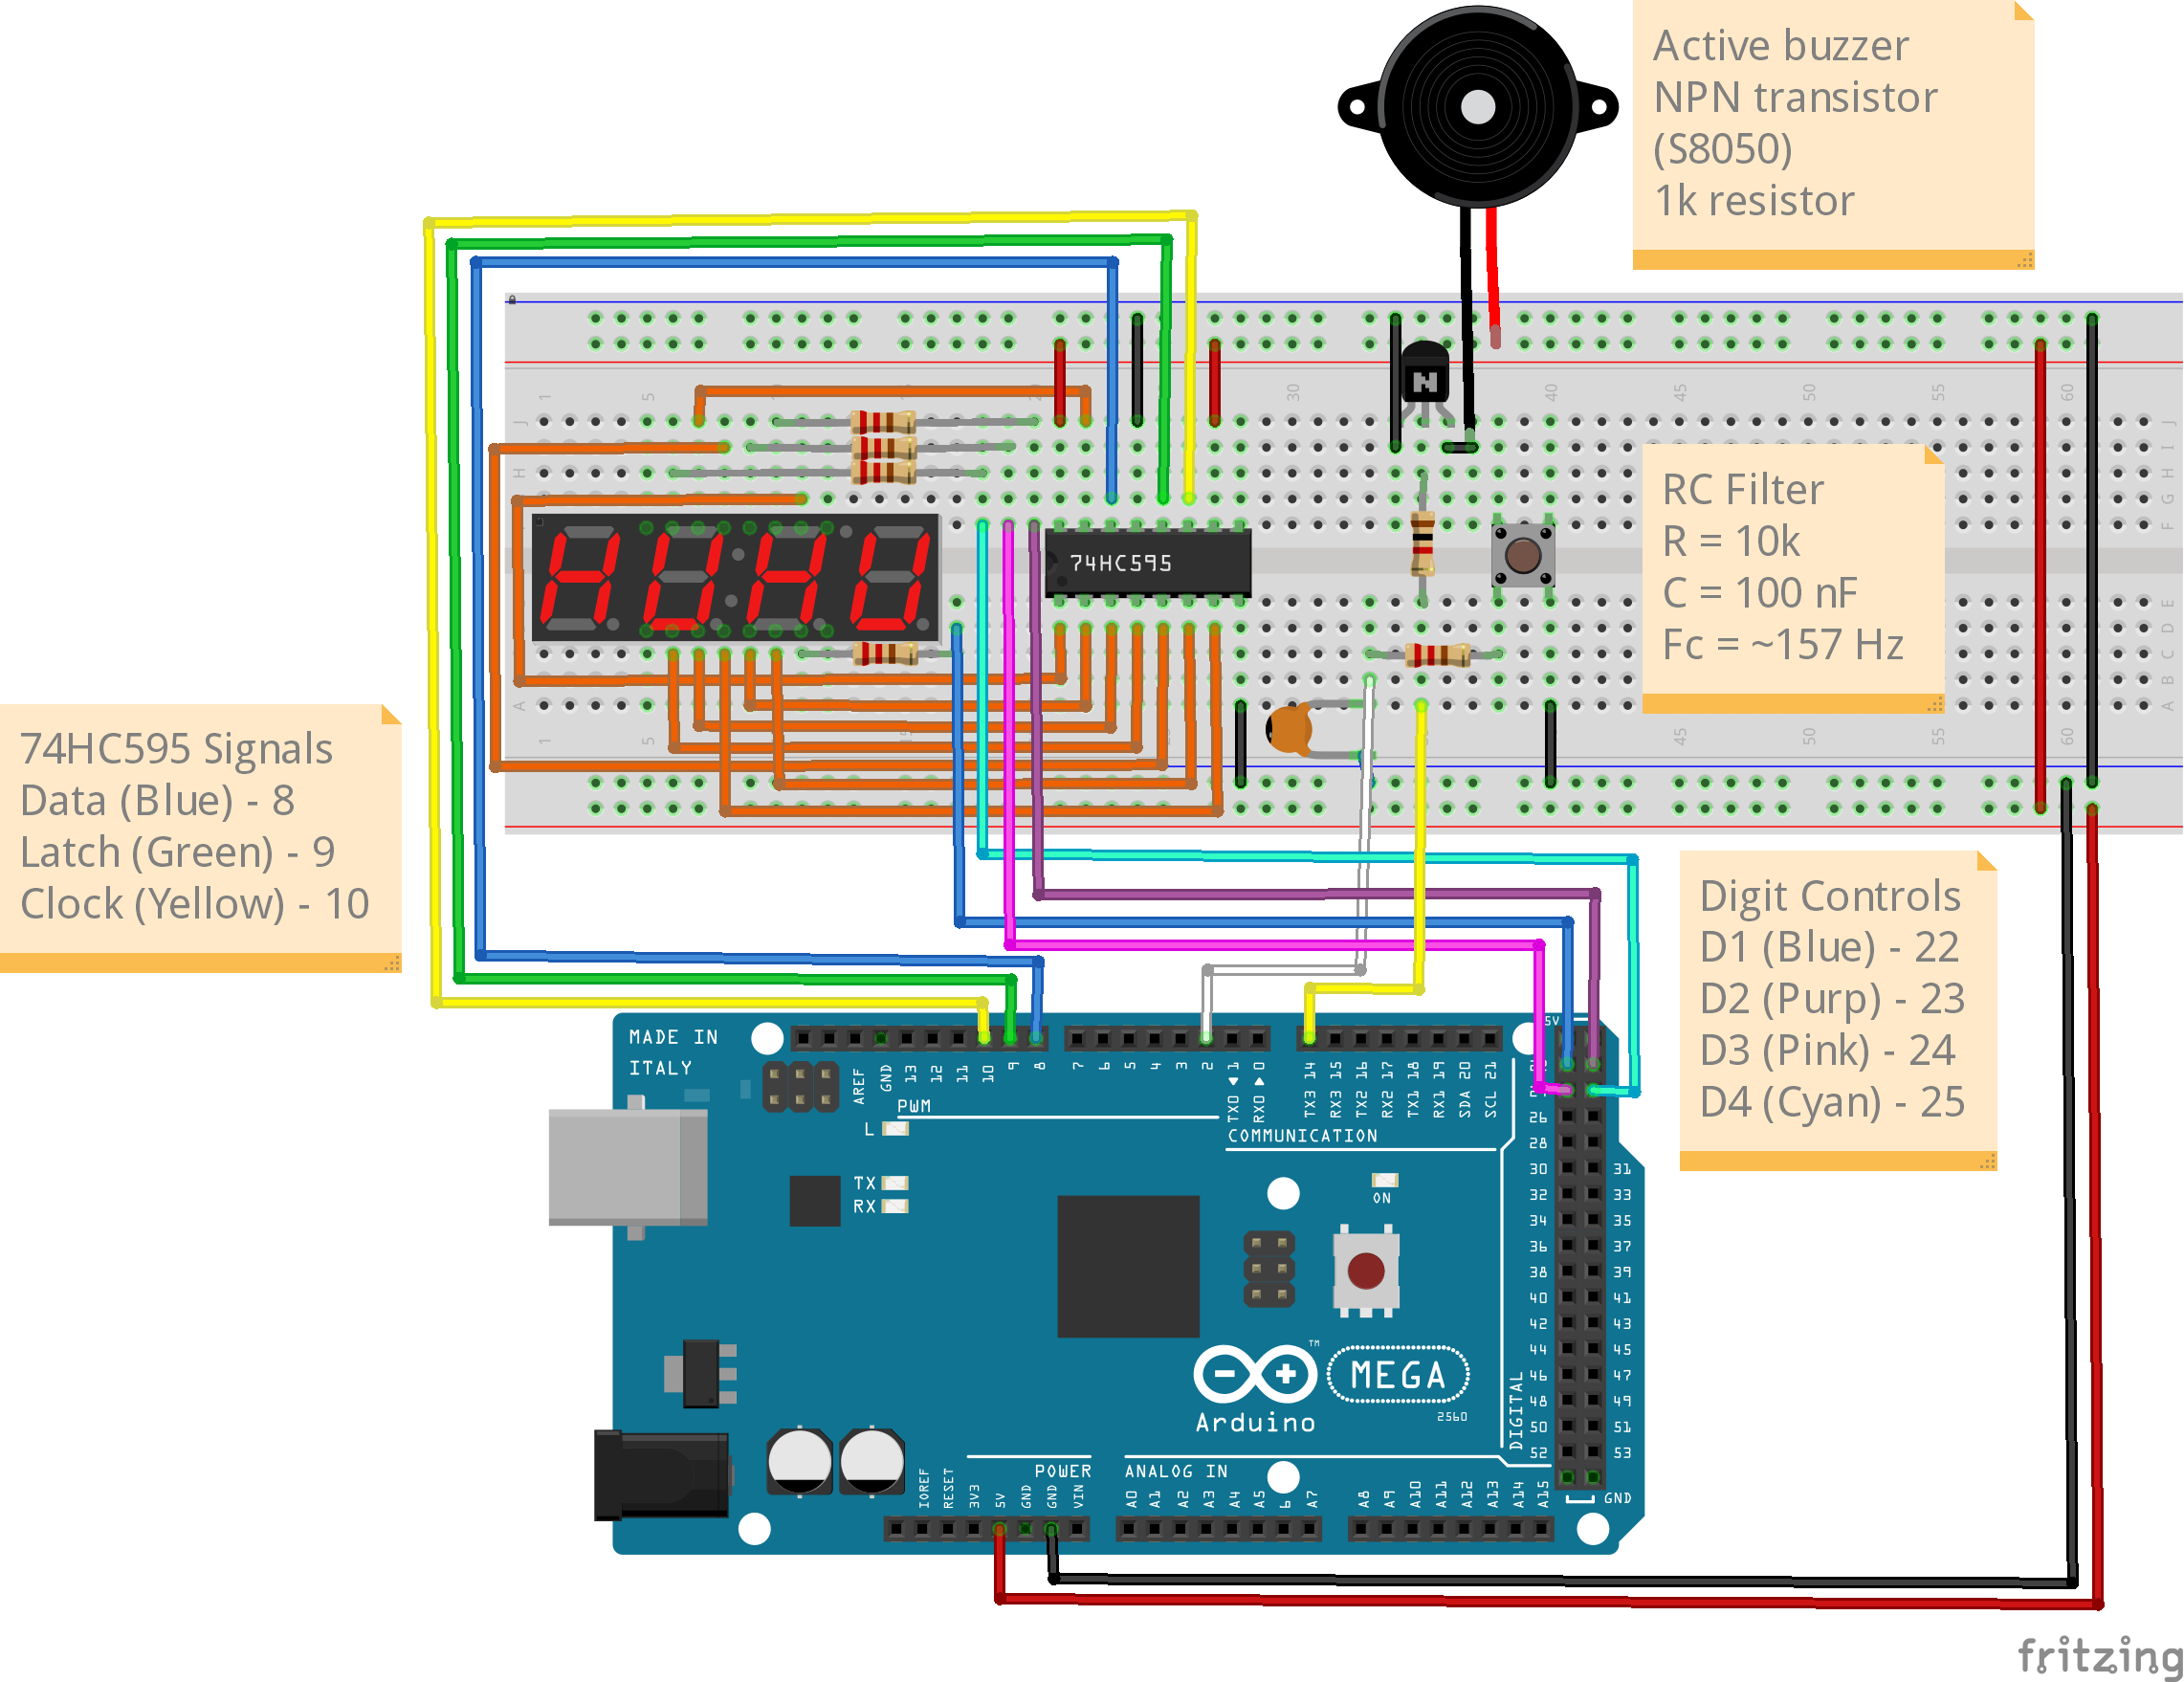
\includegraphics[height=3.5in]{../.secret/project_3_7seg_counter/p3_7seg_counter_ugrad_bb.png}
    \end{figure*}

\pagebreak

\pagelayout{margin} % Restore margins

\section*{Graduate Students} \labsec{p3_grad_students}
You will wire up five (5) buttons to your Arduino as digital inputs.
Three buttons will determine the counter increment (e.g. 1, 10, 100), and two buttons will determine the increment direction (increasing or decreasing) and be attached to interrupts to trigger the counter change.
\marginnote{\emph{Reminder:} Some filtering, either software or hardware-based will be required to accurately change the counter and prevent false readings.} 
When you hold one of the size buttons and then press either the decrement or increment button, an internal counter will increase or decrease by the size specified and update the number in the 4-digit 7-segment display.
When the decrement button is held for a certain amount of time, the counter will be reset back to 0.
For each press of the decrement or increment button, you will make an active buzzer sound as audible feedback to your inputs. \emph{For extra credit:} Figure out how to play a different tone for increment or decrement.
\marginnote{The display is only capable of showing up to four non-negative digits. So the limits of your counter will be between 0 and 9999. \emph{For extra credit:} Figure out how to make it count higher.}

Since this project is a little more complicated than previous ones, the schematic has been provided. However, the coding portion is up to you.

    \subsection*{Requirements}
    For this project you will be required to have the following:
    \begin{enumerate}
        \item A button wired to an interrupt-capable input
            \begin{itemize}
                \item Three (3) of those buttons will determine how much the counter changes
                \item Two (2) of them will determine the counter's change in direction (either increment or decrement)
                \item These buttons will be attached to digital interrupts to trigger the change in the counter
                \item Each press of these buttons will sound a buzzer for auditory feedback
            \end{itemize}
        \item The current counter value will be displayed on a 4-digit, 7-segment display
    \end{enumerate}

    \subsection*{Submission}
    You will be required to submit the following on Canvas:
    \begin{enumerate}
        \item the source code file
        \item a neat and detailed schematic of your Arduino and breadboard setup (not Fritzing, "professional-looking").
        \item A "neat" breadboard where wires are easy to track, components are visible, cross jumps are minimized, and wire colors are somewhat sensible (i.e. all orange for the shift register, white for digit selectors, blue for buttons, etc.).
    \end{enumerate}

    \subsection*{Grading}
    You will be graded along the following criteria:

    \begin{margintable}[-0.5in]
        \begin{tabular}{ l | c }
            \toprule
            Criterion & Points \\

            \midrule
            Efficacy & 50 \\
            Breadboard neatness & 10 \\
            Code neatness & 20 \\
            Schematic neatness & 20 \\
            Extra credit & 10 \\

            \bottomrule
        \end{tabular}
    \end{margintable}

    If you are willing to dig in a little bit more, this project has a couple of opportunities to earn extra credit points!
    If you want to try and get the extra credit points, please let the instructor know in the submission and detail why you believe you earn the points.
